\documentclass[12pt]{article}
\usepackage{graphicx}
\usepackage[a4paper, total={7in, 9in}]{geometry}
\usepackage{titlesec}
\graphicspath{ {images/} }

\titleformat{\paragraph}
{\normalfont\normalsize\bfseries}{\theparagraph}{1em}{}
\titlespacing*{\paragraph}
{0pt}{3.25ex plus 1ex minus .2ex}{1.5ex plus .2ex}

\title{DMT - Homework 1}
\author{
        Tran Luong Bang, Juan Mata Naranjo \\
                Master in Data Science}
\date{\today}

\begin{document}
\maketitle
\newpage

\section{Part 1.1}

Before we deep dive into each of the individual datasets and their respective results we will start out by first giving a brief overview of the number of documents we have, the number of queries applied over these documents and finally the number of queries for which we have their ground truth at our disposal. We will see that the number of ground truth results we have are much less than the total number of queries. For the evaluation metrics we will assume that the queries for which we don't have ground truth don't exist (we remove them from all evaluation metrics). We will then also outline the different text-analyzer $+$ scoring-functions we have deployed.

\begin{table}[]
\centering
\begin{tabular}{|l|l|l|}
\hline
                  & Cranfield Dataset & Time Dataset \\ \hline
Num Indexed Docs  & 1400                 & 423            \\ \hline
Num Queries       & 225                 & 83            \\ \hline
Num Queries in GT & 110                 &  80           \\ \hline
\end{tabular}
\caption{Overview Table}
\label{Overview Table}
\end{table}

\begin{table}[]
\centering
\resizebox{\textwidth}{!}{%
\begin{tabular}{|p{1cm}|p{10cm}|p{10cm}|}
\hline
\textbf{Conf ID} &
  \textbf{Text Analyzer} &
  \textbf{Scoring Functions} \\ \hline
1 &
  RegexTokenizer() $|$ LowercaseFilter() $|$ StopFilter(stoplist = STOP\_WORDS) &
  scoring.MultiWeighting(scoring.Frequency(), title=scoring.BM25F(), content=scoring.TF\_IDF()) \\ \hline
2 &
  RegexTokenizer()$|$ StopFilter(stoplist = STOP\_WORDS)$|$ LowercaseFilter() $|$ StemFilter() &
  scoring.BM25F(K1=1.2, B=.75) \\ \hline
3 &
  StemmingAnalyzer(stoplist=STOP\_WORDS) &
  scoring.TF\_IDF() \\ \hline
4 &
  FancyAnalyzer() &
  scoring.BM25F(K1=2, B=.8) \\ \hline
5 &
  SimpleAnalyzer() &
  scoring.TF\_IDF() \\ \hline
6 &
  StandardAnalyzer() &
  scoring.Frequency() \\ \hline
7 &
  FancyAnalyzer() &
  scoring.MultiWeighting(scoring.Frequency(), title=scoring.TF\_IDF(), content=scoring.BM25F()) \\ \hline
8 &
  StemmingAnalyzer(stoplist=STOP\_WORDS) &
  scoring.BM25F() \\ \hline
9 &
  RegexTokenizer()$|$ StopFilter(stoplist = STOP\_WORDS)$|$ LowercaseFilter() $|$ StemFilter() &
  scoring.MultiWeighting(scoring.Frequency(), title=scoring.TF\_IDF(), content=scoring.BM25F(K1=2, B=.8)) \\ \hline
10 &
  SimpleAnalyzer() &
  scoring.BM25F(K1=1.2, B=.75) \\ \hline
11 &
  StemmingAnalyzer(stoplist=STOP\_WORDS) &
  scoring.BM25F(K1=2, B=.8) \\ \hline
12 &
  FancyAnalyzer() &
  scoring.TF\_IDF() \\ \hline
\end{tabular}}
\caption{Configuration Overview}
\label{tab:my-table}
\end{table}


\subsection{Cranfield Dataset:}

We will now continue by presenting the most relevant results on the Cranfield Dataset. The first result presented is a table containing all the configurations (ordered by the MRR evaluation metric from highest to lowest), and the R-Precision metrics:

\begin{table}[]
\centering
\begin{tabular}{|c|c|c|c|c|c|c|c|}
\hline
\multicolumn{1}{|l|}{\textbf{Conf ID}} &
  \multicolumn{1}{l|}{\textbf{MRR}} &
  \multicolumn{1}{l|}{\textbf{Mean}} &
  \multicolumn{1}{l|}{\textbf{Min}} &
  \multicolumn{1}{l|}{\textbf{1st quartile}} &
  \multicolumn{1}{l|}{\textbf{Median}} &
  \multicolumn{1}{l|}{\textbf{3rd quartile}} &
  \multicolumn{1}{l|}{\textbf{Max}} \\ \hline
11 & 0.527 & 0.273 & 0 & 0 & 0.250 & 0.429 & 1.000 \\ \hline
2  & 0.522 & 0.278 & 0 & 0 & 0.250 & 0.490 & 1.000 \\ \hline
8  & 0.522 & 0.278 & 0 & 0 & 0.250 & 0.490 & 1.000 \\ \hline
7  & 0.504 & 0.255 & 0 & 0 & 0.250 & 0.460 & 0.667 \\ \hline
9  & 0.499 & 0.260 & 0 & 0 & 0.250 & 0.500 & 1.000 \\ \hline
4  & 0.496 & 0.264 & 0 & 0 & 0.250 & 0.448 & 1.000 \\ \hline
10 & 0.475 & 0.245 & 0 & 0 & 0.250 & 0.429 & 0.667 \\ \hline
3  & 0.416 & 0.178 & 0 & 0 & 0.143 & 0.296 & 1.000 \\ \hline
12 & 0.388 & 0.177 & 0 & 0 & 0.143 & 0.286 & 1.000 \\ \hline
1  & 0.384 & 0.184 & 0 & 0 & 0.143 & 0.286 & 1.000 \\ \hline
6  & 0.303 & 0.131 & 0 & 0 & 0.000 & 0.217 & 1.000 \\ \hline
5  & 0.166 & 0.074 & 0 & 0 & 0.000 & 0.103 & 0.833 \\ \hline
\end{tabular}
\caption{MRR and R-Precision Overview}
\label{MRR}
\end{table}




\begin{center}
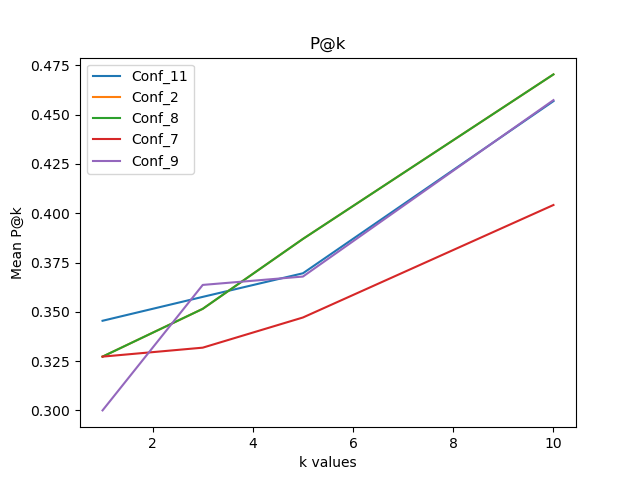
\includegraphics[scale=.75]{Pk.png}
\end{center}


\begin{center}
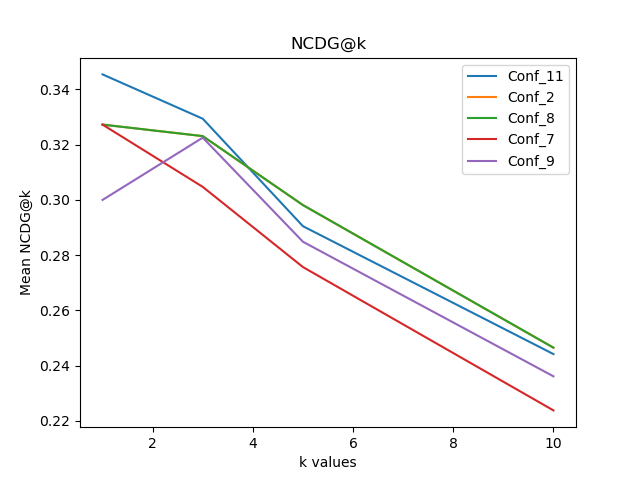
\includegraphics[scale=.75]{NCDGk.png}
\end{center}


\subsection{Time Dataset:}





\end{document}